
\subsubsection{Interface}
\label{sec:Interface}

\begin{figure}[ht]
\begin{center}
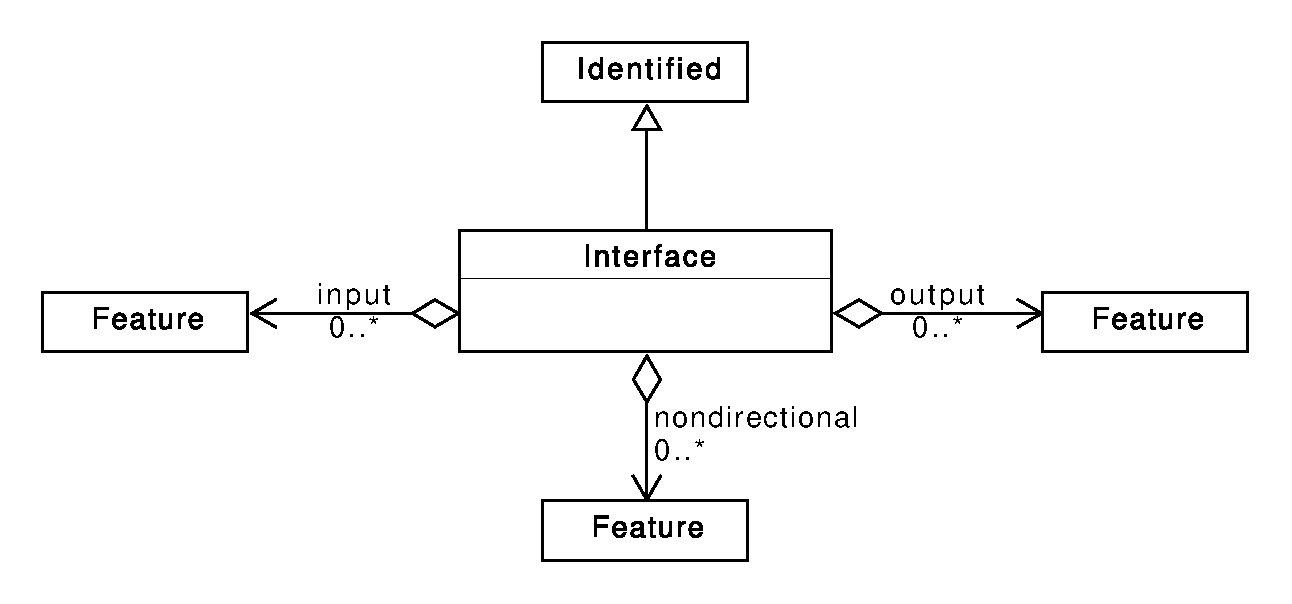
\includegraphics[scale=0.6]{uml/interface}
\caption[]{Diagram of the \sbol{Interface} class and its associated properties.}
\label{uml:interface}
\end{center}
\end{figure}

The \sbol{Interface} class is a way of explicitly specifying the interface of a \sbol{Component}. 

\subparagraph{The \sbolheading{input} property}
\label{sec:input:Interface}
The \sbolmult{input:Interface}{input} property is OPTIONAL and MAY contain a set of \sbol{Feature} \sbol{URI}s in the same \sbol{Component}.
\subparagraph{The \sbolheading{output} property}
\label{sec:output:Interface}
The \sbolmult{output:Interface}{output} property is OPTIONAL and MAY contain a set of \sbol{Feature} \sbol{URI}s in the same \sbol{Component}.

\subparagraph{The \sbolheading{nondirectional} property}
\label{sec:nondirectional:Interface}
The \sbolmult{nondirectional:Interface}{nondirectional} property is OPTIONAL and MAY contain a set of \sbol{Feature} \sbol{URI}s in the same \sbol{Component}. Note that nondirectional can imply both bidirectional as well as situations where there are no flows (for instance - a physical interface).
